\documentclass{beamer}

\title{Empirical Evaluation of the \textit{Prelude} Automatic Verification Engine with Boolean Circuits}
\author{Honors Thesis by Felix Walberg}
\date{April 15, 2026}
\begin{document}
\begin{frame}
    \titlepage 
\end{frame}
\begin{frame}
    Overview\\
    \begin{itemize}
    \item Working with MPC protocols to perform secure computations on shared data
    \item Automatically verifying these protocols are correct with \textit{Prelude} tool
    \item Testing how this tool scales as boolean circuits get larger
    \end{itemize}
\end{frame}
\begin{frame}
    Contributions\\
    \begin{itemize}
        \item \texttt{BVAdd/BVSub/BVMult/BVConcat} into \textit{Prelude} backend
        \item Parser for Bristol Circuits into \textit{Prelude} code
        \item Circuits with postconditions for Bit-Vector operations that were automatically verified
    \end{itemize}
\end{frame}
\begin{frame}
    Introduction to MPC\\
    - Motivations\\
    - Ideal functionality, no trusted 3rd party in real world\\
\end{frame}
\begin{frame}
    Introduction to MPC\\
    - What corrupt view learns\\
    - What they don't learn\\
    - Millionaires problem\\
\end{frame}
\begin{frame}
    Introduction to MPC\\
    - mpc is distributed, localized values\\ 
    - 3 party addition intro
\end{frame}
\begin{frame}
    \textit{Overture}\\
    - Language for writing MPC protocols\\
    - syntax for secrets, random values, messages, public reveal\\
    - 3 party example in Overture?\\
\end{frame}
\begin{frame}
    Correctness properties and postconditions\\
    - property for 3-party add, how we can translate that into SMT \\
\end{frame}
\begin{frame}
    Satisfiability Modulo Bit-Vector Theory\\
    - extension of SAT, searching over all bit-vector inputs\\
    - simple pythonic api example\\
    - constraints, finding solutions to pre and postcondition\\
\end{frame}
\begin{frame}
    Satisfiability Modulo Bit-Vector Theory\\
    - theorem 4.1 about entailment and e1 AND not e2 \\
\end{frame}
\begin{frame}
    \textit{Prelude} Language\\
    - metalanguage, executing \textit{Prelude} generates an \textit{Overture} MPC protocol\\
    -  2 party not xor example\\
    - circuit and prelude version\\
\end{frame}
\begin{frame}
    \textit{Prelude} Language\\
    - introduction of andgmw() with 2-bit adder\\
    - circuit first
\end{frame}
\begin{frame}
    \textit{Prelude} Language\\
    - 2 bit adder prelude\\
    - talk about post condition, how it translates well to larger circuits\\
\end{frame}
\begin{frame}
    Perl Parser\\
    - character classes to capture gate name and wires\\
    - automatic postcondition verification\\ 
\end{frame}
\begin{frame}
    Boolean circuits\\
    - 64-bit addition, subtraction, and multiplication
    - these operations in \textit{Prelude} reduces bottleneck and automatically gives us functionality\\ 
\end{frame}
\begin{frame}
    Experiments and Results\\
    - insert table\\
    \begin{figure}[h]
        \begin{center}
            \scalebox{0.8}{
        \begin{tabular}{ |c|c|c|c|c|c|}
            \hline
            & 2 party & 2-Bit & 64-Bit & 64-Bit & 64x64 -$>$ 64-Bit \\
            & NOT-XOR & Adder & Adder & Subtract & Multiplier\\
            \hline\hline
            Number of NOT gates & 1 & 0 & 0 & 63 & 0\\
            \hline
            Number of XOR gates & 1 & 3 & 313 & 313 & 9642\\
            \hline
            Number of AND gates & 0 & 1 & 63 & 63 & 4033\\
            \hline
            Total gates & 2 & 4 & 376 & 439 & 13675\\
            \hline
            \textbf{Verification time (ms)} & \textbf{21.25}& \textbf{29.75} & \textbf{4055.05} & \textbf{5931.50} & Unknown\\
            \hline
        \end{tabular}
        }
        \end{center}
        \caption{Verification times for all boolean circuits (averaged over 20 runs)}
        \label{fig-results}
        \end{figure}
\end{frame}
\begin{frame}
    Experiments and Results\\
    - insert graph\\
    \begin{figure}
        \centerline{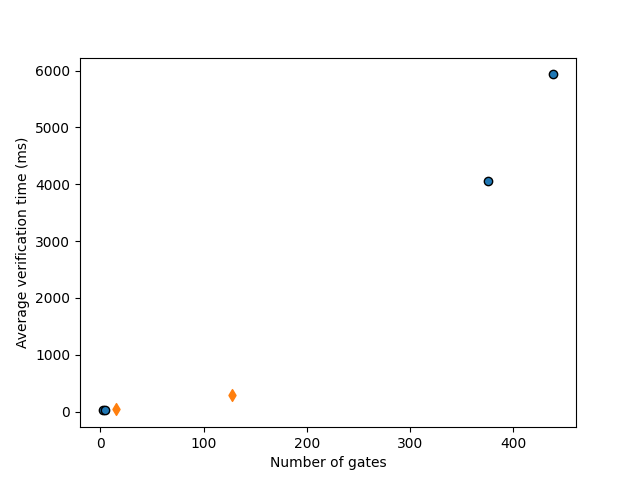
\includegraphics[scale=0.4]{../verification-graph.png}}
    \caption{Scatter plot of circuit verification time over number of gates}
    \label{verification-graph}
    \end{figure}
    - talk about roughly exponential shape\\
\end{frame}
\begin{frame}
    Conclusions and Future Work\\
    \begin{itemize}
        \item 64-bit Addition, 64-bit Subtraction verify reasonably
        \item 64-bit Multiplication posed significant challenge to the tool
    \end{itemize}
\end{frame}
\begin{frame}
    Conclusions and Future Work\\
    \begin{itemize}
    \item Extend evaluation to Yao's Garbled Circuits, which were considered in (cite both prev papers)
    \item Optimize \textit{Prelude} backend to reduce memory usage when creating constraints
    \item With reduced memory usage, attempt to verify 64-bit Multiplication, 64-bit Division
    \end{itemize}
\end{frame}
\begin{frame}
    Acknowledgements
\end{frame}
\end{document}